\rhead{22 January 2018}

\todo{again the numeration is wrong}
\underline{Reminder: }
$v_p: \Q \to \Z \cup \{\infty\} \ , \ \Z \ni z =p^k\cdot b \mapsto k$

\begin{Prop}
The discrete valuations in Ex. 1.10 are up to scaling the only discrete valuations on $\Q$.
\end{Prop}

\begin{proof}
Let $v: \Q \to \Z \cup \{\infty\}$ be a discrete valuation. Observe for $n \in \N$ we have $v(n)=v(1+\dots +1) \geq v(1)=0$. For $z \in \Z$ we have $v(z)\geq 0$, since $v(-1)=0$.
\begin{enumerate}[1)]
\item Show that $\exists p$ prime with $v(p)<0$:\\
Suppose $v(p)=0$ for all primes $p$.\\
$\Rightarrow v(n)=0$ for all $n \in \Z$.\\
$\Rightarrow v(x)=0$ for all $x \in \Q \Lightning v \not \equiv 0$
\item Observe $\a:=\{a \in \Z \ | \ v(a) >0 \}$ is an ideal in $\Z$. Use that $v(z) \geq 0$ for all $z\in \Z$.
\item Let $p$ be prime with $v(p) >0$. Such a prime exists by 1). Observe $\a=(p)$, since $p \in \a$ and $(p)$ is maximal in $\Z$. Let $c:=v(p)>0$. Denote $z \in \Z$ as $z=p^k\cdot b$ with $\gcd(b,p)=1. \Rightarrow v(z)=k \cdot v(p) + v(b) = k\cdot c$ since $v(b)=0, b\not \in (p) = \a$.
\item Obtain the result for $x \in \Q^\times$.
\end{enumerate}
\end{proof}

\begin{Bsp}
Let $K/\Q$ be a number field, $\O$ its ring of integers, $\hP_0$ a prime ideal in $\O$ above $(p)$.\\
Thm. 12 $\Rightarrow \O_{\hP_0}$ is a discrete valuation ring.\\
What is the corresponding discrete valuation on $K=\Quot(\O_{\hP_0})=\Quot(\O)$
\[v_{\hP_0}: K \to \Z \cup \{\infty\} ?\]Let $x \in K^\times \Rightarrow \underbrace{x \cdot \O}_{\text{fractional ideal}}=\hP^{e_1}_1 \cdot \ldots \dot \hP^{e_n}_n = \prod \hP \in \Spec(\O) \hP^e_{\hP} (\star)$ with $\hP_1, \ldots, \hP_n$ are prime ideals in $\O$ and $e_1, \ldots, e_n \in \Z$.\\
\underline{Claim:} $v_{\hP_0}(x)=e_{\hP_0}$.
\underline{Proof:} Consider the localisation $\O_{\hP_0}:$\\

For $\hP \neq \hP_0$ we have $\hP \cdot \O_{\hP_0} = \O_{\hP_0}.$\\
$\Rightarrow \underbrace{x \cdot \O}_{\text{fractional ideal for }\O_{\hP_0}}
 = \hP^{e_{\hP_0}}_0 \cdot \O_{\hP_0} \stackrel{(!)}{=}m^{e_{\hP_0}}$, where $m$ is the maximal ideal of $\O_{\hP_0} \Rightarrow v_{\hP_0} = e_{\hP_0}$.\\
\underline{Observe:} $v_{\hP_0}|\Q=e\cdot v_p$ where $e$ is the ramification index of $\hP_0$.
\end{Bsp}

\begin{Bsp}[Why \glqq local ring\grqq ?]
$\O=\C[X] \Rightarrow$
\begin{itemize}
\item $\O$ is noetherian $\checkmark$ 
\item $\O$ is a UFD $\Rightarrow \O$ is integrally closed $\checkmark$
\item $\O$ is a PID $\Rightarrow$ every prime ideal $\neq 0$ is maximal
\end{itemize}
$\Rightarrow \O$ is a Dedekind domain.

$\Rightarrow$
\begin{itemize}
\item $K := \Quot(\O)=\C(C)$
\item $\Spec(\O)=\{(X_z) \ | \ z \in \C\} \cup \{(0)\}$
\item $\O_{(X-z)} = \{\frac{f}{g} \in \C(X) \ | \ f,g \in \C[X], g \not \in (X-z)\}\\
\vphantom{\O_{(X-z)}} = \{\frac{f}{g} \ | \ f,g \in \C[X] , g(z) \neq 0 \}\\
\vphantom{\O_{(X-z)}} = \{\frac{f}{g} \ | \ \frac{f}{g} \text{ is definied in } z\}$\\
is a discrete valuation ring, in particular it is a local ring
\item maximal ideal $m_{(X-z)} = \{\frac{f}{g} \in \C(X) \ | \ f,g \in \C[X] \text{ with } f(z)=0, g(z) \neq 0 \} = \{\frac{f}{g} \in \C(X) \ | \ \text{ s.t. } \frac{f}{g} \text{ has a zero } in z\}$
The corresponding discrete valuation $v: \C(X) \to \Z \cup \{\infty\}$ is induced by $v: \C[X9 \setminus \{0\} \to \Z \ , \ f \mapsto \ord_z(f)= \text{ oder of zero of } f \text{ in } z = \max\{k \in \N_0 \ | \ (X-z)^k \text{ divides f}$.
\end{itemize}
\end{Bsp}

\section{Affine Schemes (Perspective}
\underline{Idea:} Link geomtreic objects to algebraic objects\\
\begin{tabular}{c c}
\underline{Geometry} & \underline{Algebra}\\
&\\
affine varietes $V$ & $\Spec(R)$\\
+&+\\
functions on $V$ & $R$
\end{tabular}

\subsection{Classical affine varieties}
\begin{defi}
Let $k$ be a field and denote $\Aff^n(k)=k^n$ (\glqq affine space\grqq)\\
$V\subseteq \Aff^n(k)$ is an \emph{\underline{affine variety}} $: \iff \exists S \subseteq k[X_1, \dots, X_n]$ s.t. $V=V(S)=\{z \in \Aff^n(k) \ | \ \forall f \in S: f(z)=0\}$.
\end{defi}

\begin{Bem}
\begin{enumerate}[i)]
\item $S_1 \subseteq S_2 \Rightarrow V(S_1) \supseteq V(S_2)$
\item Let $(S)$ be the ideal generated by $S$ in $k[X_1, \dots, X_n]$, then $V(s)=V( (S) )$.
\item Denote for $f_1, \dots, f_r: V(f_1, \dots, f_r)=V(\{f_1, \dots, f_r\})$. Every affine variety $V$ is equal to $V(f_1, \dots, f_r)$ for finitely many polynomial $f_1, \dots, f_r$ since $K[X_1, \dots, X_n]$ is noetherian.
\end{enumerate}
\end{Bem}

\begin{Bsp}
\begin{enumerate}[i)]
\item $S= \emptyset \Rightarrow V(S)=\Aff^n(k)$
\item $S=k[X_1, \dots, X_n] \Rightarrow V(S)=V(1)=\emptyset$
\item $V(X^2+Y^2-1) = $ 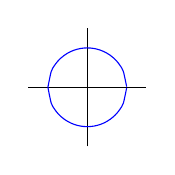
\begin{tikzpicture}[scale=0.5]
      \draw(-1.5,0) -- (1.5,0);
      \draw(0,-1.5) -- (0,1.5);
      \draw[smooth, domain=-1:1, variable=\x,blue] plot ({\x},{sqrt(1-\x*\x)});
      \draw[smooth, domain=-1:1, variable=\x,blue] plot ({\x},{-sqrt(1-\x*\x)});
    \end{tikzpicture}
\item $V(X \cdot Y) = $ \begin{tikzpicture}[scale=0.5]
      \draw[blue](-1.5,0) -- (1.5,0);
      \draw[blue](0,-1.5) -- (0,1.5);
    \end{tikzpicture}
\item $V(Y^2-X^3+X) (\leftrightarrow Y^2=X^3-X=X(X-1)(X+1))=$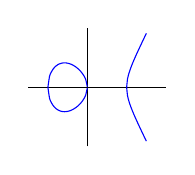
\begin{tikzpicture}[scale=0.5]
      \draw(-1.5,0) -- (2,0);
      \draw(0,-1.5) -- (0,1.5);
      \draw[smooth, domain=-1:0, variable=\x,blue] plot ({\x},{sqrt(\x*\x*\x-\x)});
      \draw[smooth, domain=1:1.5, variable=\x,blue] plot ({\x},{sqrt(\x*\x*\x-\x)});
      \draw[smooth, domain=-1:0, variable=\x,blue] plot ({\x},{-sqrt(\x*\x*\x-\x)});
      \draw[smooth, domain=1:1.5, variable=\x,blue] plot ({\x},{-sqrt(\x*\x*\x-\x)});
    \end{tikzpicture}
\item $a,b \in k \Rightarrow V(X-a, Y-b)=\{(a,b)\}$
\end{enumerate}
\end{Bsp}

\begin{Bsp}
What are the affine varieties in $\Aff^1(k)$?
\begin{itemize}
\item Rem 2.2 ii) $\Rightarrow$ sufficient to consider ideals $I$ in $k[X]$
\item Recall: Every ideal is a principal ideal, hence $I=(f)$ with $f \in k[X]$.
\end{itemize}
$\Rightarrow V(I)=\begin{cases}
\Aff^1(k), \text{ if } f = 0 \iff \deg(f)=-\infty\\
\emptyset, \text{ if } \deg(f)=0\\
\{z_1, \dots, z_k \ | \ z_i \text{ zero of } f\}, \text{ if } \deg(f) \geq 1.
\end{cases}$
\end{Bsp}

\underline{Classical goal:} Study geometry of affine varieties.\\
\underline{Idea:} Consider \glqq good\grqq classes of funtions on them.\\
Consider: (1) $k[X_1, \dots, X_n]$ as set of \emph{\underline{regular functions}} on $\Aff^n(k)=k^n$ and\\
\vphantom{Consider: } (2) $k(X_1, \dots, X_n)$ as set of \emph{\underline{rational functions}} on $\Aff^n(k)$.\\
\underline{Observe:} $f_1, f_2 \in k[X_1, \dots, X_n], V \subseteq,  \Aff^n(k), f_1 \equiv f_2$ on $V \iff f_1-f_2 \equiv 0$ on $V$.

\begin{defi}
\begin{enumerate}[i)]
\item $I(V):=\{f \in k[X_1, \dots, X_n] \ | \ \forall z \in V: f(z)=0\}$ is called \emph{\underline{vanishing ideal of $V$}}
\item $A(V):=k[V]:=k[X_1, \dots, X_n]/I(V)$ is called the \emph{\underline{$k$-algebra of regular functions of $V$}}
\end{enumerate}
\end{defi}

\begin{Bsp}
\begin{enumerate}[i)]
\item $V=\emptyset \Rightarrow I(V) = k[X_1, \dots, X_n] \Rightarrow k[V]=0$
\item $V=\{z\} \subseteq \Aff^1(k) \Rightarrow I(V)=(X-z) \Rightarrow k[V]=k[X]/(X-z)$
\item $V=\Aff^1(k), k $ infinite $\Rightarrow I(V)=(0) \Rightarrow k[V]\cong k[X]$
\item $V=\Aff^1(k), k =\F_p$ finite $\Rightarrow I(V)=(X\cdot(X-1)\cdot \ldots \cdot (X-(p-1)))$
\end{enumerate}
\end{Bsp}

\begin{Bem}
Suppose $V \subseteq \Aff^n(k)$
\begin{enumerate}[i)]
\item $I(V)$ is a radical ideal, i.e. $f^e \in I(V) \Rightarrow f \in I(V)$
\item $V(I(V)) \supseteq V$ and $I(V(I)) \supseteq I$.
\item $\bar{V}:=V(I(V))$ is the smallest affine variety containing $V$.\\
In particular, if $V$ is already an affine variety, then $V(I(V))=V$.
\item For affine varieties $V_1=V(I_1)$ and $V_2=V(I_2): V_1 \subseteq V_2 \iff I(V_1) \supseteq I(V_2)$.
In particular $V_1=V_2 \iff I(V_1)=I(V_2)$
\item $I_1 \subseteq I_2 \Rightarrow V(I_1) \supseteq V(I_2)$
\end{enumerate}
\end{Bem}